\documentclass[10pt,nocopyrightspace]{sigplanconf}

% TODO: 10pt, 11pt or nothing (default: 9pt)

\usepackage{amsmath}
\usepackage[T1]{fontenc}
\usepackage{lmodern}
\usepackage{hyperref}
\usepackage{graphicx}
\usepackage{listings}
\usepackage{subcaption}

\begin{document}

\special{papersize=8.5in,11in}
\setlength{\pdfpageheight}{\paperheight}
\setlength{\pdfpagewidth}{\paperwidth}

\titlebanner{banner above paper title}        % These are ignored unless
\preprintfooter{short description of paper}   % 'preprint' option specified.

\lstset{%
  basicstyle=\ttfamily\footnotesize,
  language=Haskell,
  frame=trBL,
  breaklines=true,
  captionpos=b,
}

\title{Hailstorm: Distributed Stream Processing with Exactly Once Semantics}
\subtitle{CS240h Final Project, Spring 2014}

\authorinfo{Thomas Dimson \and Milind Ganjoo}
           {Stanford University}
           {tdimson@cs.stanford.edu \and mganjoo@cs.stanford.edu}

\maketitle

\begin{abstract}

In recent years, \textit{stream processing} has emerged as a data analysis
technique to handle real-time applications where the latency of Hadoop is
unacceptable. Many popular systems, such as Twitter's Storm, provide a rigid
platform for performing distributed computations over the network. Storm-like
systems typically provide at-least-once processing with state management left
to the implementor. We present a novel distributed stream processing framework,
\textit{Hailstorm}\footnote{\url{https://github.com/hailstorm-hs/hailstorm}},
which is written in Haskell and provides a platform to perform distributed
computation on streams of data. By restricting the class of computation to
commutative monoids, our system is able to provide exactly-once semantics with
little performance loss or added complexity.

\end{abstract}

\section{Introduction}
\label{sec:introduction}

As the Internet has evolved so have user expectations in regards to latency.
In one example, Twitter's trending topics feature allows users to see breaking
stories within minutes of their emergence. In another, Google Analytics,
administrators are able to see detailed demographic information of surfers in
real time.  The volume and velocity of the data in these systems presents
challenges to typical single-machine programs: data does not fit into memory,
and latency requirements imply that error recovery has to be automatic and
nearly instantaneous.

Like MapReduce~\cite{mapreduce} and batch processing, frameworks such as
Twitter's Storm~\cite{storm} and LinkedIn's Samza~\cite{samza} have been
created to ease the development of stream processing applications. In these
systems, events of interest are pushed into distributed queues from user-facing
applications (e.g., Twitter's web site).  As the events are popped off the
queues, the stream processing framework takes over and transforms the event
using a sequence of computations. For example, we might receive Tweets from the
queue, split on whitespace and perform a windowed count to determine topics
that are currently trending. Similar to MapReduce, developers using these
systems write algorithms that operate on individual stream \textit{units} and
emit zero or more \textit{messages} to be handled by the next stage in
computation. The frameworks distribute the events to clusters running the
computation, abstracting away the unreliable nature of the network.

This paper introduces Hailstorm, a stream processing framework in Haskell.
Unlike Storm and Samza, Hailstorm mandates that all streaming computations must
be both commutative and monoidal. Like Samza, it requires that all events must
be initially stored as messages in Apache Kafka~\cite{kafka}.  These
restrictions allow Hailstorm to make stronger processing guarantees about
events: namely, that the each event will be processed \textit{exactly} once in
the system. Furthermore, unlike Storm and Samza, state recovery under error
conditions is built-in to the framework. We utilize Haskell's purity to
guarantee that side-effects of computation are isolated to a single
\textit{sink} processor at the end of the computation sequence.


\section{Related Work}
Hailstorm's technical design is based on that of Apache Storm~\cite{storm}.
Storm is a widely used stream processing framework for
the Java Virtual Machine (JVM) allowing developers to upload jobs for continuous
processing on a Storm cluster. Developers create a directed acyclic graph of
interconnected processing layers called a \textit{topology}.
Messages are passed between layers as
\textit{tuples}. Tuples originate in a \textit{spout}, which typically reads
off of a distributed queue and are passed between layers of \textit{bolts} which
perform computation. Each bolt receives a tuple, performs a computation, and
emits zero or more tuples to the next layer. Unlike Hailstorm, the bolts
may have side effects to their computation and state management/error recovery
is left up to each developer. Accordingly, the system is only able to provide
``at least once'' guarantees for processing each message in the queue. On
component failure, Storm enters a ``tuple replay'' state where it re-sends
messages from spouts in a topology.

The theoretical underpinings of Hailstorm are inspired by a online essay,
``Exactly Once Semantics''~\cite{jackson2014}. Jackson, a contributor to the
Storm framework, describes Kafka log offsets as a vector clock for the system
state. This clock allows separate processors to perform synchronized snapshots
without locking or direct communication. We further describe the offset clock
in Section~\ref{sec:clock}.

Google's MillWheel system~\cite{millwheel} also addresses the issue of exactly
once delivery of messages in a stream processing context. Like Storm,
messages flow through layers of computation to end up at a final result.
MillWheel provides exactly-once semantics by maintaining set of recently
processed tuples, discarding those that have recently appeared. Users of
MillWheel are required to manually ensure that all computations are
idempotent, as system failure induces message re-delivery to the same processor.

\section{Hailstorm Overview}
\label{sec:overview}

\begin{figure}
\centering
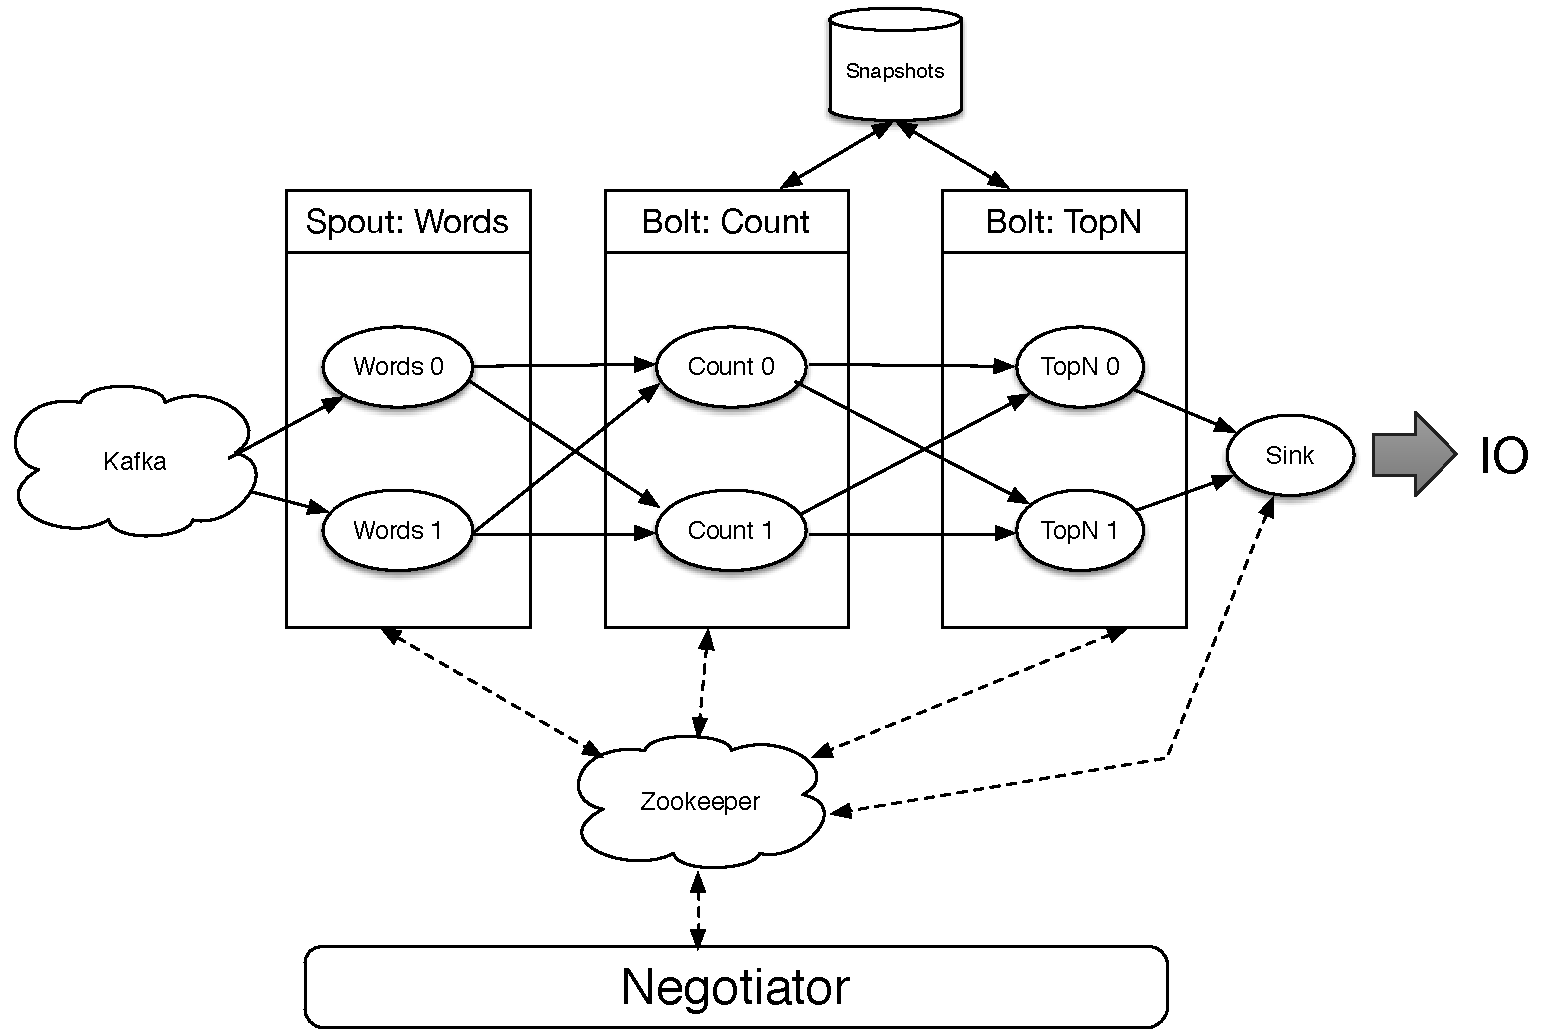
\includegraphics[width=0.5\textwidth]{images/architecture.pdf}
\caption{An example Hailstorm topology for word counts}
\label{fig:topology}
\end{figure}

Figure~\ref{fig:topology} shows a complete example of a Hailstorm system used
to calculate trending hashtags in real-time using the Twitter firehose. We give
a brief overview of the various components and describe them in detail in the
upcoming sections.

\begin{description}
\item[Apache Kafka] is used as the sole queuing mechanism for
  messages. Messages are consumed off of Kafka \textit{partitions} and then
  entered into Hailstorm along with their \textit{offset} within the
  partition.

\item[Spouts] are responsible for getting data into Hailstorm. Along
  with a user-specified conversion function, they consume \lstinline{ByteStrings}
  from Kafka and forward them as tuples to the next layer of computation.

\item[Bolts] are the fundamental units of computation in Hailstorm.
  Bolts take a user-specified pure monoidal operation which takes a (state, input-tuple)
  pair and produces a (state, output-tuple) pair. Bolt state is periodically
  persisted to the snapshot store. Figure~\ref{fig:topology} shows multiple
  layers of bolts.

\item[Sinks] are the final stage of Hailstorm processing. Like bolts,
  sinks take tuples from the previous layer and perform user-specified computation.
  However, unlike bolts, the computation runs inside the IO monad allowing the
  user to connect Hailstorm to the real world: databases, web services or even the
  console.

\item[Topologies] are user-specified directed acyclic graphs which
  describe how bolts, spouts and sinks connect together.

\item[Grouping functions] are functions that produce a hash value for a
given input tuple. When emitting a tuple to the next layer in the topology, a
processor uses the hash value to determine which instance of the target
processor to send a tuple to. For example, if a bolt has 3 instances, and a
spout emits a tuple $t$ whose hash under the bolt's grouping function $g(t)$ is
$2 \pmod 3$, then the tuple will be emitted to the third instance (index 2) of
the target bolt.

\item[Apache Zookeeper] is used as a global service registry for
  Hailstorm. Processors are registered as into Zookeeper and removed whenever
  failures occur.

\item[The negotiator] in Hailstorm manages the state of a topology: it is
  responsible for negotiating tuple snapshots and performing error recovery. The
  negotiator itself maintains no state: if it dies, it can be resumed on any
  machine with no data loss.
\end{description}

\subsection{Apache Kafka}
\begin{figure}
  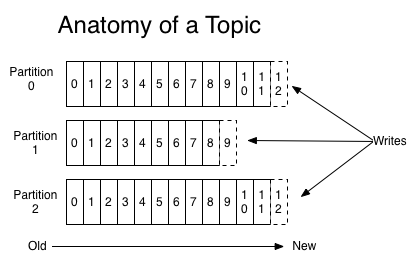
\includegraphics[width=0.45\textwidth]{images/kafka_log.png}
  \caption{Structure of Kafka partitions}\label{fig:kafka}
\end{figure}
Apache Kafka~\cite{kafka} is a distributed commit log that is used to buffer data between
producing systems (e.g., the Twitter Firehose) and Hailstorm topologies. As
described in~\ref{sec:clock}, Hailstorm requires the use of Kafka so it can
guarantee exactly-once processing of messaages. Messages are committed to
specific \textit{topics}, each with many \textit{partitions}. Within each
partition, commits are guaranteed to be linearly ordered according to time, with
Kafka providing an offset for each message. Figure~\ref{fig:kafka}, from the
Kafka website, shows the anatomy of a single topic as writes get fanned out to
different partitions. Consumers, such as Hailstorm spouts, are able to read from
individual partitions with a topic and consume mesages. Since the messages are
structured in a log, it is possible to ``rewind'' consumers and have them read
messages from earlier points in the log. Kafka also has a configerable replication
mechanism and is able to maintain its ordering even in the event of machine failure.

The latest version of the Kafka protocol lacks bindings for Haskell, however the
librdkafka~\cite{rdkafka} library provides up-to-date bindings for C. As part
of completing Hailstorm, we created the \textit{Haskakafka}\footnote{%
\url{http://hackage.haskell.org/package/haskakafka}} library that exposes
librdkafka through Haskell's C FFI\@. We have since made the bindings available on
Hackage for others to use.


\subsection{Apache Zookeeper}
\label{sec:zookeeper}
Apache Zookeeper~\cite{zookeeper} is a highly-available distributed
configuration service, which Hailstorm uses extensively for process
registry and synchronization. Zookeeper's data model is roughly analogous
to a tree-structured file system, where \textit{nodes} can either be
directories or small files. Nodes are either created indefinitely
or registered as \textit{ephemeral nodes}, which are automatically
deleted when their creator's connection is terminated. Most Zookeeper
libraries also implement \textit{watchers} on nodes which allow a program to be
asynchronously notified whenever a node or a node's data changes.

When a Hailstorm processor starts up, it immediately registers an ephemeral node
with its identifier underneath a Zookeeper directory called
\lstinline{living_processors}. As described in Section~\ref{sec:negotiator}, the
negotiator monitors this directory to ascertain the health of the system.

Hailstorm uses the hzk library~\cite{hzk}, which exposes the
Zookeeper C library to Haskell. The watcher notifications in Hailstorm occur in
a seperate (OS) thread, which communicates the value of the change
back to the worker thread using an MVar\footnote{See \texttt{ZKCluster.hs}}.

\subsection{Spouts}

\textit{Spouts}\footnote{See \texttt{Spout.hs}} are the starting point for any
flow of information through the Hailstorm system. Each spout has a one-to-one
connection with a Kafka partition.

When specifying the topology, a client provides a pure function that converts a
Kafka message to a tuple in a suitable form for processing by downstream
processors (see Listing~\ref{lst:spout-defn}).  For example, a simple ``word
count'' topology could convert a word from Kafka into a \textit{(word, 1)}
tuple to facilitate counting in downstream bolts.

Along with the tuple itself, a spout also sends a (partition, offset) pair
corresponding to the origin of the tuple. This forms the \texttt{Payload}, 
used in downstream processors for making snapshots (see \ref{sec:updating-state}).

\begin{lstlisting}[caption=Client interface for a
spout,label=lst:spout-defn,float]
data Spout =
  Spout { -- ...
        , convertFn :: BS.ByteString -> PayloadTuple
        , -- ...
        }
\end{lstlisting}

\subsubsection{Clock}
\label{sec:clock}

% TODO: I don't like the placement here, but this sets up the concept of a
% clock for later so it's important that it precedes all the remaining
% sections.
We define the notion of a vector \textit{clock} that determines the 
state of all processors regardless of message ordering.  Put
simply, the clock is a map of Kafka partition names to offset values.
More formally, a clock $C$ will contain an offset
$C[p]$ for each Kafka partition $p$ that feeds the topology.

Hailstorm uses clocks to ensure safe error recovery for processors, 
as outlined in the following sections.

\subsection{Bolts}
\label{sec:bolts}

Bolts\footnote{See \texttt{Downstream.hs}} form the computational portion of
the Hailstorm topology. Each bolt maintains an internal state (represented by
the type \lstinline{BoltState}), which is updated as the computation advances.
The key characteristic of Hailstorm bolt states is that they are commutative
monoids\footnote{This is not enforced. It is the client's responsibility to
  provide a \lstinline{mergeFn} definition that performs a commutative
  \lstinline{mappend} between two \lstinline{BoltState} instances.}.  This
  allows any state to be represented as a \lstinline{mappend} of one or more
  older states. Commutativity ensures that ordering of messages is unimportant
  to the final result. Monoids have important implications for crash recoverability:
  a snapshot of an older state allows computations to start 
  from that point forward instead of starting from scratch.

A subset of the client-provided bolt interface is shown in
Listing~\ref{lst:bolt-defn}. Incoming tuples are converted to a monoidal
\lstinline{BoltState} to facilitate merging with the existing state. The
conversion is performed using \lstinline{tupleToStateConverter} (a function
that converts a key-value pair into a singleton map would be an example). The
\lstinline{mergeFn} performs commutative \lstinline{mappend}. The tuples
themselves are transformed using the new state and
\lstinline{transformTupleFn}) and forwarded downstream.

\begin{lstlisting}[caption=Client interface for a
bolt,label=lst:bolt-defn,float]
data Bolt =
  Bolt { -- ...
       , transformTupleFn :: PayloadTuple -> BoltState -> PayloadTuple
       , emptyState :: BoltState
       , mergeFn :: BoltState -> BoltState -> BoltState
       , tupleToStateConverter :: PayloadTuple -> BoltState
       -- ...
       }
\end{lstlisting}

\subsubsection{Updating state with incoming tuples}
\label{sec:updating-state}

Incoming tuples are always merged into the existing bolt state. Depending on
whether the negotiator has posted a desired snapshot clock (see
Section~\ref{sec:negotiator}), this could involve either one or two states:

\begin{itemize}

  \item When there is no snapshot being requested, incoming tuples are merged
  into a single state instance. The output tuple from a bolt is calculated
  using this single state.

  \item When a bolt receives a negotiator request to perform a snapshot, it
  splits its current state into state $A$ and $B$: its current state becomes
  $A$ and it initializes $B$ to \lstinline{mempty}.

  \item As long as the bolt is not eligible to perform a snapshot (see
  Section~\ref{sec:lwm} for when this is determined), the bolt maintains two
  states: pre-snapshot state $A$ and post-snapshot state $B$. It merges tuples
  into the appropriate state based on their source partition offsets, and
  calculates the downstream tuple based on a combination of these two states.
  More formally, for a desired snapshot clock $C$, if an incoming tuple
  originated from partition $p$ at offset $o$, then the tuple will be merged
  into state $A$ if $o \leq C[p]$; otherwise, it is merged into $B$. The
  downstream output tuple will be calculated from $A + B$.

  \item When it is time to actually persist its state, the bolt forks a thread
  to persist pre-snapshot state $A$. In the main thread, it merges states $A$
  and $B$ and merges new tuples into this single state, reverting to the
  no-snapshot phase.

\end{itemize}

\subsubsection{Low Water Mark}
\label{sec:lwm}

After the snapshot request is received and a bolt bifurcates its state, it must
wait till the pre-snapshot state is guaranteed to no longer be affected by
incoming tuples. To help determine when this happens, bolts use another piece
of information: the \textit{low water mark (LWM)}.

A low water mark $LWM_k$ for a processor $k$ is simply a clock (see
Section~\ref{sec:clock}), where offset $LWM_k[p]$ for partition $p$ is the
\emph{lowest} offset seen by any processor upstream to $k$. It is calculated
recursively (as shown in Figure~\ref{fig:lwm-calculation}), and indicates the
\emph{least} amount of progress made for each partition in the entire topology.

\begin{figure}
  \begin{subfigure}[t]{0.45\columnwidth}
    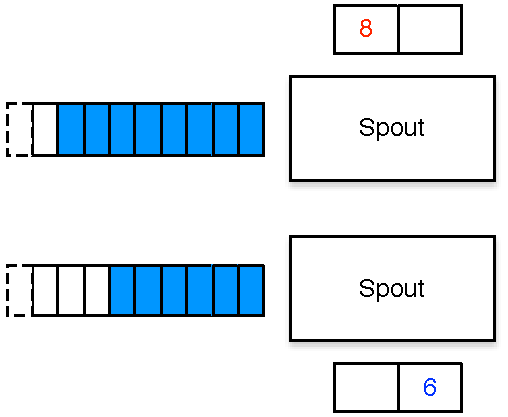
\includegraphics[width=\columnwidth]{images/lwm_spouts.pdf}
    \caption{LWM for a spout has just one entry: the offset in the associated
    partition.}
  \end{subfigure}
  \hfill%
  \begin{subfigure}[t]{0.45\columnwidth}
    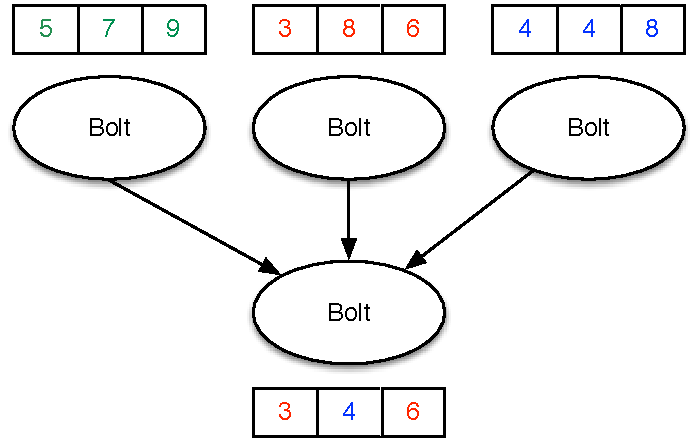
\includegraphics[width=\columnwidth]{images/lwm_bolts.pdf}
    \caption{LWM for a bolt is calculated as $min(LWM_k)$ for each upstream
    $k$.}
  \end{subfigure}
  \caption{Calculating LWM for processors.}\label{fig:lwm-calculation}
\end{figure}

To help downstream bolts calculate their LWMs, payloads carry a map
of upstream processor names to their respective LWMs, which is updated at each
level.

The LWM is used in determining snapshot eligibility as follows: a bolt may only
persist its state when its LWM equals the desired snapshot clock in
\emph{every} dimension. When that happens, future tuples are guaranteed to
originate from offsets greater than ones in the desired snapshot clock, and
thus the pre-snapshot state for a bolt will no longer change.

\subsubsection{Saving and restoring snapshots}
\label{sec:snapshot}

Bolts receive an instance of a \lstinline{SnapshotStore} typeclass with two
functions: \lstinline{saveSnapshot} and \lstinline{restoreSnapshot}. When a
bolt is eligible to snapshot its state, it forks a thread to perform the save.
On boot-up, a bolt tries to restore its state from the provided
\lstinline{SnapshotStore}. If there is nothing saved, it starts from an empty
state.

In the current Hailstorm implementation, we provide a
\lstinline{DirSnapshotStore} instance that creates a snapshot in a local
directory. Ideally, one would want to provide other instances: one that uses an
SQL database, or one that uses a distributed file system for greater fault
tolerance.

\subsection{Sinks}

Sinks are at the bottom-most level of a topology. As the final computation
step, they serve the role of gateway to the real world. Sinks often perform
actions like printing to console or writing to a database (they are the only
processors in the topology that are allowed to execute impure code). The user
action is provided by the client in the form of a Pipes \lstinline{Consumer}
that accepts upstream tuples (see Listing~\ref{lst:sink-defn}).

There is no restriction to the type of computation performed on incoming
tuples; however, since no snapshots are performed on sinks, non-idempotent
operations may have unexpected results.

\begin{lstlisting}[caption=Client interface for a
sink,label=lst:sink-defn,float]
data Sink =
  Sink { -- ...
       , outputConsumer :: Consumer PayloadTuple IO ()
       , -- ...
       }
\end{lstlisting}

\subsection{Negotiator}
\label{sec:negotiator}

The \textit{negotiator}\footnote{See \texttt{Negotiator.hs}} has full control
over all the processors of a Hailstorm topology. The negotiator shares
two related roles:
\begin{enumerate}
  \item Forcing bolts to snapshot with a valid clock
  \item Recovering the state of the system if a processor
        becomes unreachable
\end{enumerate}

Upon registration, the negotiator creates a special ephemeral node for the
topology called the \textit{master state}. The negotiator transitions the master
state through the deterministic finite automaton shown in
Figure~\ref{fig:masterstate}. Each processor in the topology creates a
watcher for the master state, responding quickly to transitions.

\begin{figure}[h]
  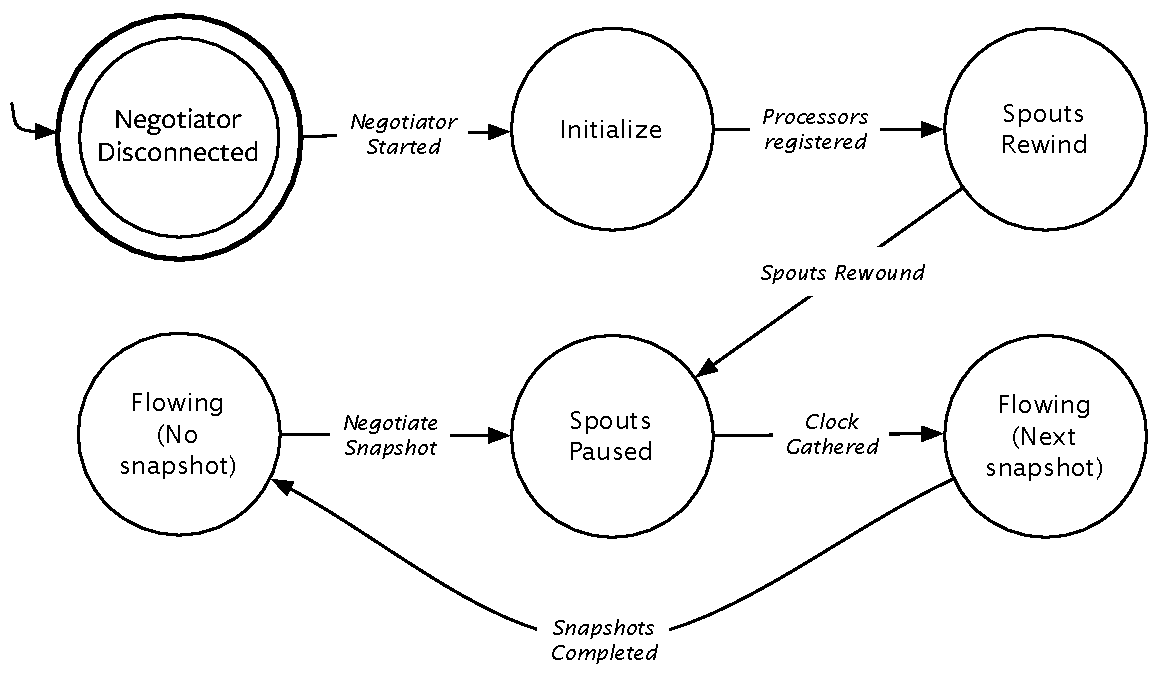
\includegraphics[width=0.45\textwidth]{images/master_state.pdf}
  \caption{Master state machine for a topology. After initialization, the
  topology loops between flowing and making snapshots
  indefinitely.}\label{fig:masterstate}
\end{figure}

Initially, the topology begins in the \lstinline{NegotiatorDisconnected} state which
is indicated by the absence of a master state node in Zookeeper. When the
negotiator boots up, it sets the master state to \lstinline{Initialize} and waits
for all processors to register under living processors (see
Section~\ref{sec:zookeeper}). Once the expected nodes have been created, the
negotiator waits for the bolts to load their snapshots from the snapshot store
(see Section~\ref{sec:snapshot}). The bolts communicate their snapshot clock
their living processor nodes, and negotiator is then able change the master state to
\lstinline{SpoutsRewind}. The spouts rewind to the clock, and pause, writing their
position into their corresponding living processor nodes. Finally, the
negotiator begins the main \textit{run loop}.

Hailstorm's run loop consists of the negotiator alternating between snapshots
and a grace period of data flow. When data is flowing without a desired snapshot
clock, the negotiator sets the master state to \lstinline{Flowing Nothing} and
then waits a configerable grace period. After the grace period expires, the
negotiator sets the state to \lstinline{SpoutsPaused} and determines the next
snapshot clock from the current spout offsets. When complete, the negotiator sets
the master state to \lstinline{Flowing NextClock}, which the bolts use to determine
their snapshot. After the bolt snapshots are complete, the negotiator returns to
\lstinline{Flowing Nothing} and loops.

The run loop can be interrupted by an unreachable processor. When a processor
becomes unresponsible, their Zookeeper connection terminates and their
corresponding ephemeral node is removed from the living processors directory.
The negotiator is asynchronously notified through a watcher, and then sets the
master state to \lstinline{Initialize}. As part of this transition, the negotiator
removes the living processor nodes for all processors in the topology. Each
processor reads this as a signal to restart, so that the topology can restart in
a clean state. Thus the \lstinline{Initialize} master state is identical to that of
the negotiator's initial start.

\section{Example Topology}
In light of the technical details of Section~\ref{sec:overview}, we return to the
sample topology of Figure~\ref{fig:topology}. The topology uses 
Hailstorm to calulate trending hashtags in real-time from Twitter
\footnote{See \texttt{Sample/WordCountSample.hs}}. In a non-distributed setting,
the computation would typically use the unix \texttt{sort} and \texttt{uniq}
commands. Hailstorm enables the same principles to scale to datasets far beyond a
single computer's memory.

On the producer side, we enqueue messages into Kafka using a Python script. The script
samples hashtags from the Twitter's web API and then enqueues them into Kafka as 
UTF-8 bytestrings .

As data streams into Kafka, Hailstorm streams data out. The spouts
take the UTF-8 bytestrings, convert them into Haskell character lists
and send them to the next layer of \textit{count} bolts. Our hashing function, 
the native Haskell string hash, forces a 1:1 mapping betweem hashtag and bolt instance. 
For example, \#love, would always be mapped to \textit{count-0}.

The \textit{count} bolts aggregate individual hashtag occurrences into a running
sum. This running sum is stored as a hash map 0 default value, making each addition 
a monoidal operation. Hashtags are received, aggregated, and emitted with the running count.
For example, \textit{count-0} could receive \texttt{(\#love,1)} and emit
\texttt{(\#love, 101)} to the next layer of \textit{topn} bolts.

Each \textit{topn} bolt keeps track of the local top $n$ trending hashtags 
that have been sent to it. The computation utilizes the Haskell PSQueue
library~\cite{psqueue}, implementing a pure keyed priority queue. Each hashtag
is added to the queue, which is then trimmed to the top $n$ entries. The entire
queue is sent to the next (and final) layer for processing.

In the sample topology, the \textit{sink} receives the local top $n$ queues 
and merges them to compute the global top $n$ hashtags. Finally, the top $n$
tags are emitted to the console. The action occurs in the IO Monad and could be 
modified to update a database or website as appropriate.

\section{Implementation Details}

\subsection{Running Processors}

Each of the processors in the topology (spouts, bolts and sinks) can be run
independently, as long as they are uniquely identifiable (such as through
unique port numbers). The \texttt{HailstormCLI.hs} sample executable included
with the library allows such behavior, with processors runnable on different
threads, cores, or machines.

\subsection{Network Processing}
\label{sec:network-processing}
Hailstorm utilizes the Haskell Pipes~\cite{pipes} library
in place of Lazy I/O. Within
a processor, the next layer is modeled as a \lstinline{Pool} consumer%
\footnote{See \texttt{Processor/Pool.hs}} that keeps a connection pool
of downstream processor sockets. The \lstinline{Pool} consumer waits for a
Hailstorm \lstinline{Payload}, hashes it, and then sends it via a network socket
\lstinline{Handle}. Handles themselves are lazily created and maintained within a
connection pool. In our initial implementation, messages are serialized using
Haskell's \texttt{Show} method; we intend to migrate to a more efficient
protocol in upcoming versions.

Bolt and spout layers listen for incoming connections and process their
messages. After initialization, they instantiate a \textit{mailbox} using the
Pipes-Concurrency~\cite{pipes-concurrency} library and fork a listener
thread\footnote{See \texttt{Processor/Downstream.hs}}. The listener thread
accepts upstream connections and forks handlers that push incoming tuples
into the mailbox. The main processor thread creates a Pipes pipeline that
consumes messages from the mailbox, processes them in a pipes
and then sends output to a consumer (\lstinline{Pool} for bolts,
IO for sinks).

\section{Next Steps}
Our Hailstorm implementation is functionally complete, but could use some
polishing before a public release.

Currently, the only the \lstinline{HardcodedTopology} data type conforms to the the
\lstinline{Topology} type-class. Accordingly, a user of Hailstorm has to program
the network port and address for each processor into the Hailstorm binary
itself. A modification to Hailstorm would register each the network address
in the Zookeeper processor registry. The modification would allow processors to
be resumed on different machines then they started on.

In that direction, we would like to structure the framework closer to a Hadoop
cluster wherein developers upload \textit{jobs} to Hailstorm. We envision
developers ``uploading'' their processors into Zookeeper, with Hailstorm
executing the specification. The framework would utilize a package like
hint~\cite{hint} to provide dynamic code execution from Zookeeper.

\section{Conclusion}
% TODO: make this better
This paper introduces Hailstorm, a Storm-like distributed stream processing
framework for Haskell. By restricting our class of computation to commutative
monoids and by exploiting Haskell's purity, the system guarantees exactly-once
processing of messages without performance loss. Hailstorm maintains these
guarantees even in the face of machine failures and an unreliable network. We
look forward to developing it further.

\bibliography{hailstorm}{}
\bibliographystyle{abbrvnat}

\end{document}
